\documentclass[main-ap-physics.tex]{subfiles}
\usetikzlibrary{decorations.markings}

\begin{document}

\begin{center}
    \begin{tikzpicture}
        \begin{axis}[width=6cm,height=6cm,
            xmin=0,xmax=11,
            ymin=0,ymax=11,
            axis lines=center,
            xlabel={$x$},
            ylabel={$y$},
            clip=false,
            xtick={0,1,...,9},
            ytick=\empty,
            xticklabels={},
        ]
        \draw[ultra thick,violet,->] (0,0) -- ++(9,0) node[pos=0.2,above,black] {$\theta = \ang{0}$} node[pos=0.7,above=2pt,black] {9 units};
        \end{axis}
    \end{tikzpicture}%
    \hspace{2em}
    \begin{tikzpicture}
        \begin{axis}[width=6cm,height=6cm,
            xmin=0,xmax=11,
            ymin=0,ymax=11,
            axis lines=center,
            xlabel={$x$},
            ylabel={$y$},
            clip=false,
            xtick={9},
            ytick=\empty,
            xticklabels={},
        ]
        \draw[ultra thick,violet,->] (0,0) -- ++(9,0);
        \draw[ultra thick,violet,->] (9,0) -- ++(0,5);
        \end{axis}
    \end{tikzpicture}%
    \hspace{2em}
    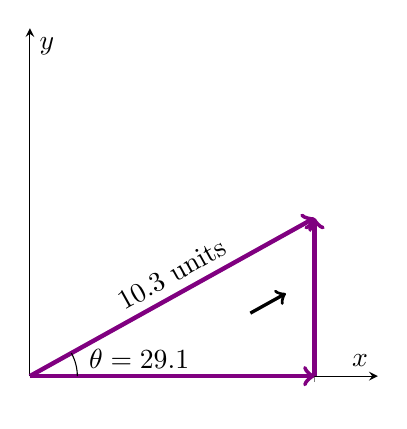
\begin{tikzpicture}
        \begin{axis}[width=6cm,height=6cm,
            xmin=0,xmax=11,
            ymin=0,ymax=11,
            axis lines=center,
            xlabel={$x$},
            ylabel={$y$},
            clip=false,
            xtick={9},
            ytick=\empty,
            xticklabels={},
        ]
        \draw[ultra thick,violet,->] (0,0) -- ++(9,0);
        \draw[ultra thick,violet,->] (9,0) -- ++(0,5);
        \draw[ultra thick,violet,->] (0,0) -- (9,5) node[pos=0.75,above left,rotate=29.1,black] {10.3 units};
        \draw (1.5,0) arc (0:29.1:1.5) node[pos=0.75,right=2pt] {$\theta = \ang{29.1}$};
        \end{axis}
    \tkzRegle[Fond=true,Opacite=0.9,CouleurFond=yellow,AfficheValeurs=false,Origine={(0.2,1.2)},Echelle=0.3,Rotation=29.1]
        \tkzRapporteur[Fond,CouleurFond=blue,Echelle=0.1,Origine={(2.8,0.8)},AfficheAngles=false]
        \draw[very thick,->] (2.8,0.8) -- ++(0.05*9,0.05*5);
    \end{tikzpicture}
    \captionsetup{type=figure,margin=1in,font=scriptsize}
    \captionof{figure}{\textbf{Head-to-Tail Method}: The head-to-tail method of graphically adding vectors is illustrated for the two displacements of the person walking in a city considered in Figure ?.??. (a) Draw a vector representing the displacement to the east. (b) Draw a vector representing the displacement to the north. The tail of this vector should originate from the head of the first, east-pointing vector. (c) Draw a line from the tail of the east-pointing vector to the head of the north-pointing vector to form the sum or \textbf{resultant vector} $\textbf{D}$. The length of the arrow $\textbf{D}$ is proportional to the vector’s magnitude and is measured to be 10.3 units . Its direction, described as the angle with respect to the east (or horizontal axis) $\theta$ is measured with a protractor to be \ang{29.1}.}
\end{center}

\textbf{Step 1}. \textit{Draw an arrow to represent the first vector (9 blocks to the east) using a ruler and protractor.}

\begin{center}
    \begin{tikzpicture}
        \begin{axis}[width=6cm,height=6cm,
            xmin=0,xmax=11,
            ymin=0,ymax=11,
            axis lines=center,
            xlabel={$x$},
            ylabel={$y$},
            clip=false,
            xtick={0,1,...,9},
            ytick=\empty,
            xticklabels={},
        ]
        \draw[ultra thick,violet,->] (0,0) -- ++(9,0) node[pos=0.2,above,black] {$\theta = \ang{0}$} node[pos=0.7,above=2pt,black] {9 units};
        \end{axis}
    \end{tikzpicture}
\end{center}

\textbf{Step 2}. Now draw an arrow to represent the second vector (5 blocks to the north). \textit{Place the tail of the second vector at the head of the first vector}.

\begin{center}
    \begin{tikzpicture}
        \begin{axis}[width=6cm,height=6cm,
            xmin=0,xmax=11,
            ymin=0,ymax=11,
            axis lines=center,
            xlabel={$x$},
            ylabel={$y$},
            clip=false,
            xtick={9},
            ytick=\empty,
            xticklabels={},
        ]
        \draw[ultra thick,violet,->] (0,0) -- ++(9,0);
        \draw[ultra thick,violet,->] (9,0) -- ++(0,5);
        \end{axis}
    \end{tikzpicture}
\end{center}

\textbf{Step 3}. \textit{If there are more than two vectors, continue this process for each vector to be added. Note that in our example, we have only two vectors, so we have finished placing arrows tip to tail.}

\vspace{1em}

\textbf{Step 4}. \textit{Draw an arrow from the tail of the first vector to the head of the last vector}. This is the resultant, or the sum, of the other vectors.

\begin{center}
    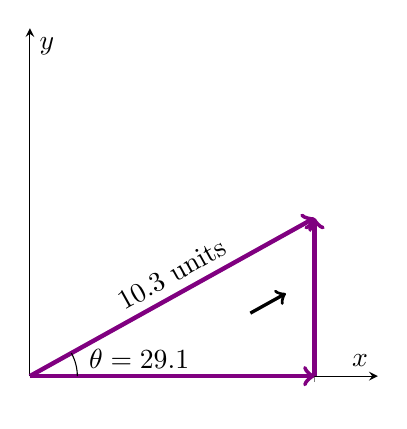
\begin{tikzpicture}
        \begin{axis}[width=6cm,height=6cm,
            xmin=0,xmax=11,
            ymin=0,ymax=11,
            axis lines=center,
            xlabel={$x$},
            ylabel={$y$},
            clip=false,
            xtick={9},
            ytick=\empty,
            xticklabels={},
        ]
        \draw[ultra thick,violet,->] (0,0) -- ++(9,0);
        \draw[ultra thick,violet,->] (9,0) -- ++(0,5);
        \draw[ultra thick,violet,->] (0,0) -- (9,5) node[pos=0.75,above left,rotate=29.1,black] {10.3 units};
        \draw (1.5,0) arc (0:29.1:1.5) node[pos=0.75,right=2pt] {$\theta = \ang{29.1}$};
        \end{axis}
    \tkzRegle[Fond=true,Opacite=0.9,CouleurFond=yellow,AfficheValeurs=false,Origine={(0.2,1.2)},Echelle=0.3,Rotation=29.1]
        \tkzRapporteur[Fond,CouleurFond=blue,Echelle=0.1,Origine={(2.8,0.8)},AfficheAngles=false]
        \draw[very thick,->] (2.8,0.8) -- ++(0.05*9,0.05*5);
    \end{tikzpicture}
\end{center}

\textbf{Step 5}. \textit{To get the magnitude of the resultant, measure its length with a ruler. (Note that in most calculations, we will use the Pythagorean theorem to determine this length.)}

\vspace{1em}

\textbf{Step 6}. \textit{To get the direction of the resultant, measure the angle it makes with the reference frame using a protractor. (Note that in most calculations, we will use trigonometric relationships to determine this angle.)}

\vspace{1em}

The graphical addition of vectors is limited in accuracy only by the precision with which the drawings can be made and the precision of the measuring tools. It is valid for any number of vectors.

\begin{example}
    \textit{Adding Vectors Graphically Using the Head-to-Tail Method: A Woman Takes a Walk}. Use the graphical technique for adding vectors to find the total displacement of a person who walks the following three paths (displacements) on a flat field. First, she walks \SI{25.0}{m} in a direction  \ang{49.0} north of east. Then, she walks \SI{23.0}{m} heading \ang{15.0} north of east. Finally, she turns and walks \ang{32.0}{m} in a direction \ang{68.0} south of east.
\end{example}

\Solution \textit{Strategy}: Represent each displacement vector graphically with an arrow, labeling the first $\textbf{A}$, the second $\textbf{B}$, and the third  $\textbf{C}$, making the lengths proportional to the distance and the directions as specified relative to an east-west line. The head-to-tail method outlined above will give a way to determine the magnitude and direction of the resultant displacement, denoted $\textbf{R}$.

\vspace{1em}

(1) Draw the three displacement vectors.

\begin{center}
    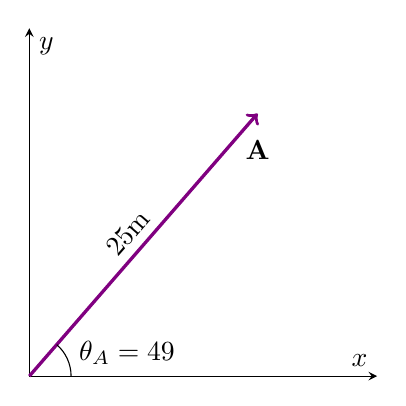
\begin{tikzpicture}
        \begin{axis}[width=6cm,height=6cm,
            xmin=0,xmax=25,
            ymin=0,ymax=25,
            clip=false,
            ylabel=$y$,
            xlabel=$x$,
            ticks=none,
            axis lines=center
        ]
        \draw[very thick,->,violet] (0,0) -- ({25*cos(49)},{25*sin(49)}) node[pos=0.6,black,above left,rotate=49] {\SI{25}{m}} node[black,below=2mm] {$\textbf{A}$};
        \draw (3,0) arc (0:49:3) node[pos=0.7,right=2pt] {$\theta_{\text{A}} = \ang{49}$};
        \end{axis}
    \end{tikzpicture}%
    \hspace{2em}
    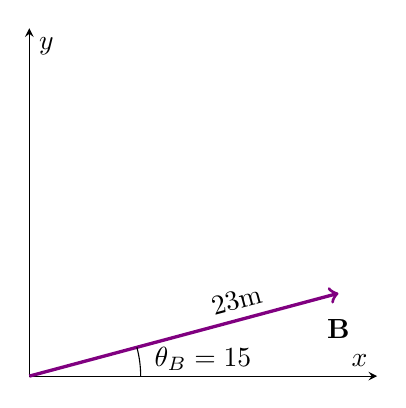
\begin{tikzpicture}
        \begin{axis}[width=6cm,height=6cm,
            xmin=0,xmax=25,
            ymin=0,ymax=25,
            clip=false,
            ylabel=$y$,
            xlabel=$x$,
            ticks=none,
            axis lines=center
        ]
        \draw[very thick,->,violet] (0,0) -- ({23*cos(15)},{23*sin(15)}) node[pos=0.8,black,above left,rotate=15] {\SI{23}{m}} node[black,below=2mm] {$\textbf{B}$};
        \draw (8,0) arc (0:15:8) node[pos=0.6,right=2pt] {$\theta_{\text{B}} = \ang{15}$};
        \end{axis}
    \end{tikzpicture}%
    \hspace{2em}
    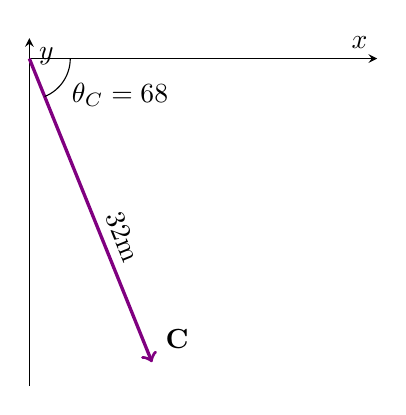
\begin{tikzpicture}
        \begin{axis}[width=6cm,height=6cm,
            xmin=0,xmax=34,
            ymin=-32,ymax=2,
            clip=false,
            ylabel=$y$,
            xlabel=$x$,
            ticks=none,
            axis lines=center,
            clip=false,
        ]
        \draw[very thick,->,violet] (0,0) -- ({32*cos(-68)},{32*sin(-68)}) node[pos=0.5,black,above right,rotate=-68] {\SI{32}{m}} node[black,above right=1pt] {$\textbf{C}$};
        \draw (4,0) arc (0:-68:4) node[pos=0.08,right=-1mm] {$\theta_{\text{C}} = \ang{68}$};
        \end{axis}
    \end{tikzpicture}
\end{center}

(2) Place the vectors head to tail retaining both their initial magnitude and direction.

\begin{center}
    \begin{tikzpicture}
    
        \begin{axis}[width=12cm,height=6cm,
            xmin=0,xmax=60,
            ymin=0,ymax=30,
            axis lines=center,
            ticks=none,
            clip=false,
            ylabel=$y$,
            xlabel=$x$,
            clip=false,
        ]
        \coordinate (A) at ({25*cos(49)},{25*sin(49)});
        \coordinate (B) at ({23*cos(15)},{23*sin(15)});
        \coordinate (AB) at ({25*cos(49)+23*cos(15)},{25*sin(49)+23*sin(15)});
        \coordinate (C) at ({32*cos(-68)},{32*sin(-68)});
        \coordinate (R) at ({50.8*cos(-5.47)},{50.8*sin(-5.47)});
        
        \draw[very thick,violet,->] (0,0) -- (A) node[black,pos=0.5,below=1mm] {$\textbf{A}$};
        \draw[very thick,violet,->] (A) -- ++(B) node[pos=0.5,black,below=1mm] {$\textbf{B}$};
        \draw[very thick,violet,->] (AB) -- ++(C) node[pos=0.5,black,right=1mm] {$\textbf{C}$};
        \end{axis}
    \end{tikzpicture}
\end{center}

(3) Draw the resultant vector,  $\textbf{R}$.

\begin{center}
    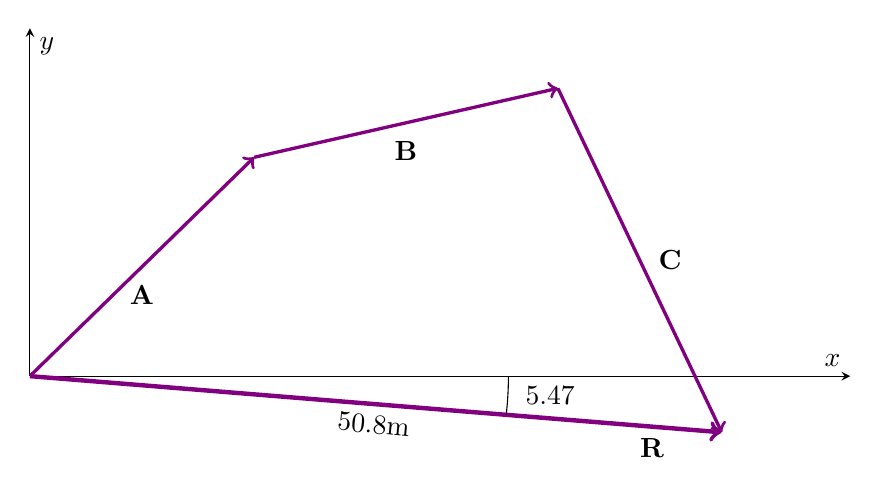
\begin{tikzpicture}
        \begin{axis}[width=12cm,height=6cm,
            xmin=0,xmax=60,
            ymin=0,ymax=30,
            axis lines=center,
            ticks=none,
            clip=false,
            ylabel=$y$,
            xlabel=$x$,
            clip=false,
        ]
        \coordinate (A) at ({25*cos(49)},{25*sin(49)});
        \coordinate (B) at ({23*cos(15)},{23*sin(15)});
        \coordinate (AB) at ({25*cos(49)+23*cos(15)},{25*sin(49)+23*sin(15)});
        \coordinate (C) at ({32*cos(-68)},{32*sin(-68)});
        \coordinate (R) at ({50.8*cos(-5.47)},{50.8*sin(-5.47)});
        
        \draw[very thick,violet,->] (0,0) -- (A) node[black,pos=0.5,below=1mm] {$\textbf{A}$};
        \draw[very thick,violet,->] (A) -- ++(B) node[pos=0.5,black,below=1mm] {$\textbf{B}$};
        \draw[very thick,violet,->] (AB) -- ++(C) node[pos=0.5,black,right=1mm] {$\textbf{C}$};
        \draw[ultra thick,violet,->] (0,0) -- (R) node[black,pos=0.5,below,rotate=-5.47] {\SI{50.8}{m}} node[pos=0.9,below,black] {$\textbf{R}$};
        \draw (35,0) arc (0:-5.47:35) node[pos=0.5,right=1mm] {\ang{5.47}};
        \end{axis}
    \end{tikzpicture}
\end{center}

(4) Use a ruler to measure the magnitude of $\textbf{R}$, and a protractor to measure the direction of $\textbf{R}$. While the direction of the vector can be specified in many ways, the easiest way is to measure the angle between the vector and the nearest horizontal or vertical axis. Since the resultant vector is south of the eastward pointing axis, we flip the protractor upside down and measure the angle between the eastward axis and the vector.

\begin{center}
    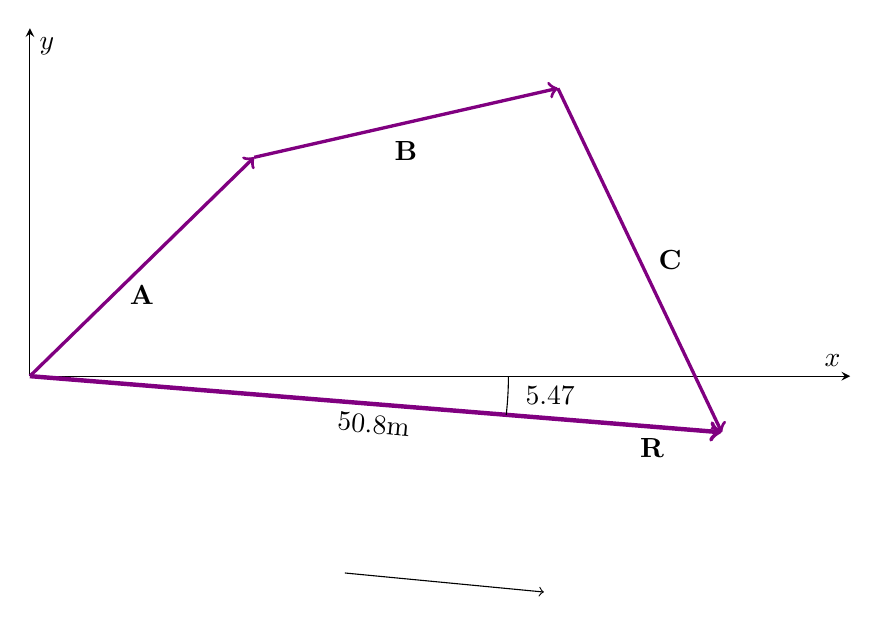
\begin{tikzpicture}
    
        \begin{axis}[width=12cm,height=6cm,
            xmin=0,xmax=60,
            ymin=0,ymax=30,
            axis lines=center,
            ticks=none,
            clip=false,
            ylabel=$y$,
            xlabel=$x$,
            clip=false,
        ]
        \coordinate (A) at ({25*cos(49)},{25*sin(49)});
        \coordinate (B) at ({23*cos(15)},{23*sin(15)});
        \coordinate (AB) at ({25*cos(49)+23*cos(15)},{25*sin(49)+23*sin(15)});
        \coordinate (C) at ({32*cos(-68)},{32*sin(-68)});
        \coordinate (R) at ({50.8*cos(-5.47)},{50.8*sin(-5.47)});
        
        \draw[very thick,violet,->] (0,0) -- (A) node[black,pos=0.5,below=1mm] {$\textbf{A}$};
        \draw[very thick,violet,->] (A) -- ++(B) node[pos=0.5,black,below=1mm] {$\textbf{B}$};
        \draw[very thick,violet,->] (AB) -- ++(C) node[pos=0.5,black,right=1mm] {$\textbf{C}$};
        \draw[ultra thick,violet,->] (0,0) -- (R) node[black,pos=0.5,below,rotate=-5.47] {\SI{50.8}{m}} node[pos=0.9,below,black] {$\textbf{R}$};
        \draw (35,0) arc (0:-5.47:35) node[pos=0.5,right=1mm] {\ang{5.47}};
        \end{axis}
        \tkzRegle[Fond=true,Opacite=0.9,CouleurFond=yellow,AfficheValeurs=false,Origine={(0.2,-0.6)},Echelle=0.6,Rotation=-5.47]
        \tkzRapporteur[Fond,CouleurFond=blue,Echelle=0.4,Origine={(4,-2.5)},AfficheAngles=false,Rotation=-180]
        \draw[->] (4,-2.5) -- ++ ({0.05*50.8*cos(-5.47)},{0.05*50.8*sin(-5.47)});
    \end{tikzpicture}
\end{center}

In this case, the total displacement $\textbf{R}$ is seen to have a magnitude of \SI{50.8}{m} and to lie in a direction  \ang{5.47} south of east. By using its magnitude and direction, this vector can be expressed as $\textbf{R} = \SI{50.8}{m}$ and $\theta = \ang{5.47}$ south of east.

\vspace{1em}

\textbf{Discussion}: The head-to-tail graphical method of vector addition works for any number of vectors. It is also important to note that the resultant is independent of the order in which the vectors are added. Therefore, we could add the vectors in any order as illustrated in Figure \ref{ondDEl} and we will still get the same solution.

\begin{center}
    \begin{tikzpicture}
        \begin{axis}[width=12cm,height=6cm,
            xmin=0,xmax=60,
            ymin=0,ymax=30,
            axis lines=center,
            ticks=none,
            clip=false,
            ylabel=$y$,
            xlabel=$x$,
            clip=false,
        ]
        \coordinate (A) at ({25*cos(49)},{25*sin(49)});
        \coordinate (B) at ({23*cos(15)},{23*sin(15)});
        \coordinate (AB) at ({25*cos(49)+23*cos(15)},{25*sin(49)+23*sin(15)});
        \coordinate (C) at ({32*cos(-68)},{32*sin(-68)});
        \coordinate (CA) at ({32*cos(-68)+25*cos(49)},{32*sin(-68)+25*sin(49)});
        \coordinate (R) at ({50.8*cos(-5.47)},{50.8*sin(-5.47)});
        
        \draw[very thick,violet,->] (0,0) -- (C) node[black,pos=0.5,below left] {$\textbf{C}$};
        \draw[very thick,violet,->] (C) -- ++(A) node[pos=0.5,black,below right] {$\textbf{A}$};
        \draw[very thick,violet,->] (CA) -- ++(B) node[pos=0.4,black,below right] {$\textbf{B}$};
        \draw[ultra thick,violet,->] (0,0) -- (R) node[black,pos=0.5,below,rotate=-5.47] {\SI{50.8}{m}} node[pos=0.9,above,black] {$\textbf{R}$};
        \draw (35,0) arc (0:-5.47:35) node[pos=0.5,right=1mm] {\ang{5.47}};
        \end{axis}
    \end{tikzpicture}
\end{center}

Here, we see that when the same vectors are added in a different order, the result is the same. This characteristic is true in every case and is an important characteristic of vectors. Vector addition is commutative. Vectors can be added in any order.

\begin{equation}
    \textbf{A} + \textbf{B} = \textbf{B} + \textbf{A}
\end{equation}

(This is true for the addition of ordinary numbers as well---you get the same result whether you add $2+3$ or $3+2$, for example).

\endsolution

 



\end{document}



